\chapter{Game Development}
\label{chap:game_development}

\section{Fasi dello sviluppo}

I lavori sul progetto ``The Magic Lantern'' sono iniziati a cavallo di Gennaio e Febbraio, dove i primi meeting con l'azienda sono serviti per spiegare i retroscena del progetto e il documento di game design iniziale.
Al secondo meeting è stata definitiva una timeline per l'intero lavoro, in buona parte rispettata. 

La timeline ha previsto una divisione del lavoro in due macro sezioni, dove in ognuna delle quali sono stati portati a termine vari sotto-fasi ed obiettivi:

\begin{itemize}

\item Pre Production: periodo stimato (Febbraio-Marzo)

\begin{itemize}
\item High Concept revision: all'inizio è servito rivedere il concept iniziale, recepire i feedback ricevuti dalla commissione Europea (per la quale il progetto si era precedentemente iscritto) e quindi riformulare, tramite varie sessioni di brainstorming, un nuovo concept.
\item Pitch: rielaborato il concept, si è spiegato tutto in un breve pitch, per definire bene i nuovi intenti di design.
\item Concept art revision: oltre al concept di gameplay si è fatto un concept anche a livello artistico.
\item Game Design Document updating: una volta approvato il pitch e le varie revisioni, l'obiettivo è stato quello di riscrivere il documento di game design.
\item Prototyping: definito il documento di design, si è creato un prototipo che confermi in prima battuta le scelte di design prese. Questi ultimi 2 step sono stati ripetuti più volte.
\end{itemize}

\item Production: periodo stimato (Aprile-Luglio)

\begin{itemize}
\item Game Design: una volta scelto il Game Design definitivo dalla fase precedente, questo è stato rivisto e ulteriormente raffinato.
\item Development: a questo punto, lo sviluppo vero e proprio della demo definitiva è partito.
\item Level Design: una grossa parte della production è stata dedicata al level design, in quanto, una volta creato un gameplay di base, è servito studiare come farlo fruire al giocatore.
\item Art production: a questo punto è stato necessario il supporto dal reparto grafico al fine di ``colorare'' e ``riempire'' il mondo di gioco. In genere gli artisti forniscono concept al resto del team al fine di fornire anche nuove idee per livelli e ambientazioni varie. In questo caso specifico, il reparto artistico ha fornito gli asset indispensabile per rendere il gioco chiaro e minimamente godibile.
\item Audio production: per ogni sezione di gioco è stato inserito il relativo audio, al fine di trasmettere le sensazioni volute al player.
\item First Playable: dopo aver tenuto conto di tutti i focus precedenti, si è passati alla creazione della prima versione giocabile della demo.
\item Testing alpha version: finalizzata la demo giocabile, questa va testata tramite il pubblico target, quindi vanno analizzati i risultati e i feedback raccolti.
\end{itemize}

\end{itemize}

(*********)

La fase di Pre-Production è stata, in buona parte, rispettata. La fase di Production, invece, è stata ritardata di qualche settimana per via delle vacanze Pasquali e altre rielaborazioni varie che hanno riguardato le ultimi due focus del pre-production (Game Design Document e Prototyping), in quanto è stato necessario provare più volte versioni dei design pensati (come è solito per ogni videogame che attraversa questa fase). Qui sono state fatte varie prove di gameplay, tentando varie combinazioni di comandi dello strumento centrale del gioco, la Lanterna Magica. Come già detto nel capitolo di Game Design (**********), si è inoltre scelto di concentrare il gioco soprattutto sulle meccaniche intorno alla Lanterna, piuttosto che dare un uguale peso ad altre tecnologie del pre-cinema, se così non fosse stato, si sarebbero create troppe combinazioni e la complessità del gioco si sarebbe elevata troppo, considerati anche il tempo e i mezzi a disposizione. Si è scelto quindi di utilizzare le altre tecnologie in altri modi, come per esempio mini livelli o comunque sezioni limitate di gioco. In generale, questa fase ha visto un largo studio dello stato dell'arte dei giochi di interesse per il nostro studio, giochi sia di tipo Serious Game sia di tipo platform e puzzle. Si è quindi cercato di prendere spunto dai pattern più famosi al fine di rendere il gioco il più comprensibile possibile.

La fase di Production, iniziata a fine Aprile, ha visto una fetta enorme di tempo dedicata al level design. Non è stato facile definire un livello di difficoltà per il pubblico target, ma in generale per il giocatore. In questa fase ci si è scontrati con dei veri problemi di design, e si è cercato di capire come una meccanica andrebbe fornita al player. Per fare ciò, ci si è ispirati in parte anche ai giochi esposti nella sezione dello stato dell'arte (*********). Dopo una lunga fase, durante la quale sono stati usati dei placeholder, è arrivato il supporto grafico per rendere il gioco più chiaro e adatto per un generico pubblico, questo supporto è arrivato a Giugno (nonostante fosse stato preventivato verso Aprile-Maggio). A causa di vari ritardi, come quello del supporto grafico, ma anche l'implementazione dei livelli finali e le modalità di fruizione dei contenuti Serious, la fase di Production (della demo) non si è potuta concludere a Luglio, come stabilito, in quanto si è riusciti a portare a termine solo il primo round di testing, mentre era necessario farne almeno un secondo per apportare le modifiche necessarie in base ai feedback ricevuti durante il primo round, e quindi capire valutare l'efficacia dei cambiamenti applicati. Ovviamente, prima dei test esterni, sono state svolte varie sedute di testing interno all'azienda, per capire se il prodotto fosse pronto per un pubblico esterno.


\section{Strumenti}

The Magic Lantern è stato implementato tramite il game engine Unity3d versione 5.1.1.f1 (\url{https://unity3d.com}) usando prevalentemente il linguaggio di programmazione C\#. Unity3d è un game engine che fornisce un editor molto user-friendly, col quale si può familiarizzare anche in poche ore. Esistono moltissimi tutorial sul web riguardo Unity3d.

Come sistema di versioning è stato utilizzato Git (******** biblio), tramite il programma SourceTree che fornisce una interfaccia grafica molto facile da utilizzare.

E' stato utilizzato inoltre, come strumento di team management e comunicazione interna, il programma Asana. Questo è uno strumento molto utile per assegnare task e fissare scadenze, cose essenziali per lavorare in team.


\section{Logica implementativa di gameplay}

\section{Controller del player}

\section{Lanterna Magica e vetrini}


\section{AI e spawner}

Poiché il gioco prevede l'interazione con dei nemici, è stato necessario sviluppare una logica di AI. Poiché il comportamento designato dei nemici non è molto complesso, si è scelto di utilizzare una macchina a stati come logica di base, evoluta in un secondo momento in una macchina a stati gerarchica.

E' possibile vedere un Class Diagram rappresentante dell'implementazione usata:

\begin{figure}[h]
\centerline{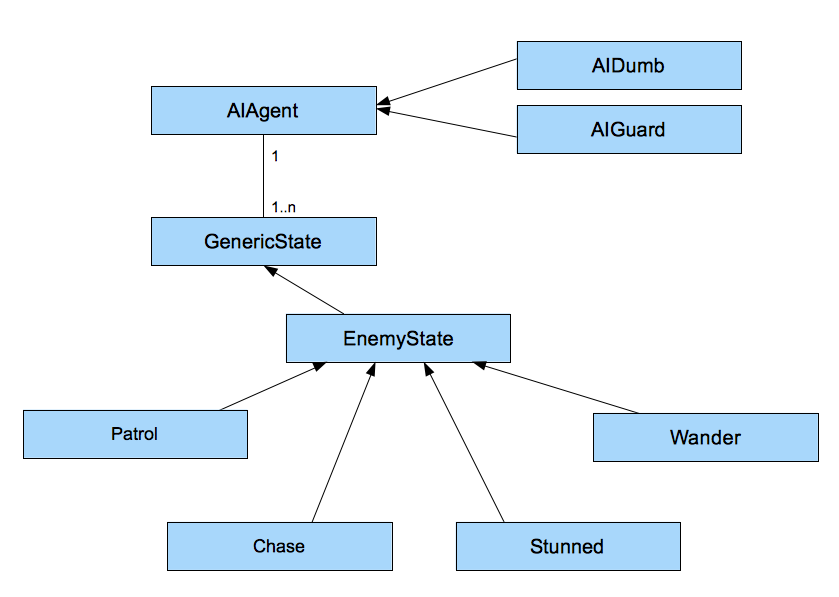
\includegraphics[scale=0.45]{images/development/classdiagramAI.png}}
\caption{Class Diagram della AI usata.}
\label{fig:classdiagramAI}
\end{figure}

Il funzionamento di questa macchina a stati da la possibilità di gestire il comportamento di uno stato a diversi livelli di profondità, nonostante nell'implementazione finale sia stato usato un livello di profondità massimo pari a 2, si può potenzialmente andare ben oltre.
L'idea è che le azioni fatte dall'AI saranno presenti sempre nelle foglie della gerarchia, cioè in quegli stati che non avranno figli, mentre gli stati intermedi, oltre che il medesimo, forniranno il supporto per il controllo di eventuali cambi di stato.
La scelta di questa logica permette una gestione ordinata dei passaggi di stato, oltre che un buon riuso del codice. Per esempio, lo stato intermedio \manclass{Patrol} può avere più stati figli sotto di sé, quali: \manclass{SuspiciousPatrol}; \manclass{WalkPatrol}; \manclass{StandPatrol}; \manclass{AreaPatrol} (nota bene, nel parlare di stati foglia, stati padre e stati figli, non si intendono concetti di ereditarietà tipica della programmazione ad oggetti). Questi ``stati foglia'', oltre che essere collegati fra loro da transizioni di stato (per esempio tutti sono collegati a SuspiciousPatrol e WalkPatrol, mentre gli altri due sono in genere esclusivi fra loro), sono tutti collegati anche ad altri stati. Quando tutti gli stati sotto lo stesso stato padre presentano la medesima transizione, allora di questa transizione è responsabile il padre, la logica di controllo è quindi definita nella classe padre, infatti, come già detto, a controllare la necessità di transizione sono sia lo stato attivo sia gli stati gerarchici sopra quello stato. Per esempio, quando il player salto in testa ad un nemico mentre si trova in uno dei suoi stati Patrol, questo passerà in ogni caso allo stato \manclass{Stunned} che gestisce la morte o il temporaneo ``intontimento'' dei nemici.

Detto ciò, l'implementazione di un nemico prevede l'uso di una classe derivata da \manclass{AIAgent}, per esempio \manclass{AIGuard} e al suo interno andranno specificati gli stati padre e figli da utilizzare (come \manclass{Patrol} e \manclass{WalkPatrol} etc). L'implementazione è basata sull'uso di delegati, invocati da \manclass{AIAgent}, in particolare sono invocati i delegati degli stati padre superiori, i quali, invocheranno in modo ricorsivo tutti i delegati fino a finire la gerarchia. 

I delegati, usati per ogni stato, sono:

\begin{itemize}

\item Initialize: invocato quando si entra nello stato dopo una transizione.
\item Finalize: invocato quando si esce dallo stato a causa di una transizione.
\item Update: invocato dallo stato attivo ogni frame, viene quindi invocato durante la funzione \manclass{Update} di \manclass{AIAgent}.
\item StateTransition: è un array di delegati che controllano se occorre effettuare una transizione di stato, vengono invocate durante la funzione \manclass{Update} di \manclass{AIAgent}, prima che venga invocato anche il delegato \manclass{Update}.
\item TriggerEnter: viene invocato quando viene invocata la funzione OnTriggerEnter2D di \manclass{AIAgent}.
\item CollisionEnter: viene invocato quando viene invocata la funzione OnCollisionEnter2D di \manclass{AIAgent}, invocata per esempio quando il nemico tocca il player o un muro.

\end{itemize}

L'implementazione scritta della macchina a stati non è ancora definitiva al 100\%, in quanto deve essere costruito uno schema che sia in grado di prevenire errori dall'errata impostazione della macchina, quindi occorre l'implementazione di metodi o di interfacce che agevolino questo compito.

Mentre il nemico ``Dumb'', non è in grado di fare delle azioni ``ragionate'', ma semplicemente cammina avanti e indietro, fin quando non trova la morte sul suo cammino (dovuta al player o all'ambiente), il secondo (la cui macchina a stati è mostrata in \myfig{\ref{fig:gerarchiaAIGuard}} ) invece presenta un minimo ragionamento, avendo degli stati che gli permettono di fare la guardia ad un posto o un area e riconoscere il player, quindi attaccarlo con un carica e ucciderlo al contatto (a meno che il contatto non avvenga sulla sua testa, in quel caso muore il Guard).

\begin{figure}[h]
\centerline{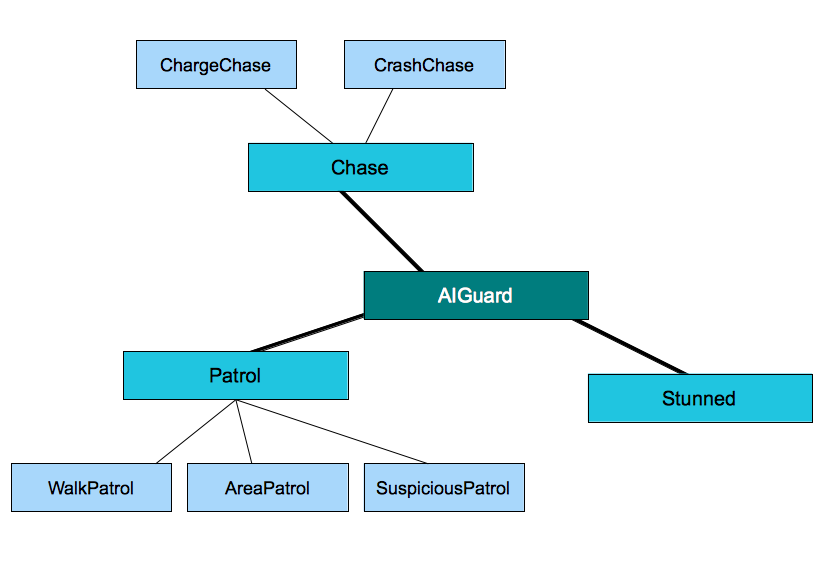
\includegraphics[scale=0.45]{images/development/gerarchiaAIGuard.png}}
\caption{Gerarchia macchina a stati del nemico ``Guard''.}
\label{fig:gerarchiaAIGuard}
\end{figure}

Infine, diciamo che correlato ai nemici, c'è lo script che gestisce la loro generazione, chiamato \manclass{spawner}. Questo genera da 1 ad n nemici, ad un ritmo di tot secondi (personalizzabile anche questo), avendo cura di controllare quanti nemici generati siano ancora in vita, così da non sforare il limite massimo scelto. Quando un nemico muore, se generato da uno spawner, richiama un metodo dell'istanza del relativo spawner, avvisando che è morto, quindi decrementando il contatore interno di nemici in vita.

\newpage

\section{Menù, schede informative e contenuti sbloccabili}

Sia il menù di pausa che l'interfaccia utente delle schede informative, sono state implementate tramite l'uso della ``UI'' di Unity3d. Gli script che regolano l'uso di entrambi sono \manclass{MenuManager} e \manclass{InformativeManager}, dove il primo gestisce il menù di pausa, mentre il secondo la navigazione dei contenuti Serious del gioco (oltre che metodi per analizzare quanto i contenuti siano stati letti, ma di questo parleremo nella sezione *********). Quando si entra in pausa, il timeScale passa a zero (una proprietà di Unity che regola lo scorrere del tempo) e si tiene traccia che non si è in gioco anche tramite una variabile statica della classe \manclass{PlayStatusTracker}, ``inPlay'', se questa è true, è attivo o il menù o l'interfaccia delle schede informative.
Il menù da la possibilità di ricominciare il livello, uscire dal gioco (e accedere alla prima scena con il menù principale) e accedere alle schede informative. La sezione di schede informative, come descritto nella sezione di design (*********), è navigabile in modo da accedere a vari contenuti con le relative immagini.

Lo sblocco di un contenuto, avviene tramite lo script \manclass{UnlockContent}, il quale comunica ad \manclass{InformativeManager} quale contenuto è stato sbloccato.

\section{GeneralFinder e Utils}

Sono stati creati degli script per agevolare e rendere più efficiente le varie logiche di gioco. Per esempio, è stato creato uno script, chiamato \manclass{GeneralFinder} che raccoglie tutti i riferimenti più importanti della scena (come \manclass{PlayerMovements}, \manclass{InformativeManager} etc) e li immagazzina in variabili statiche, in modo che se un qualunque script debba in una qualunque parte del codice, accedere allo script del player, può farlo così: \manclass{GeneralFinder.PlayerMovements}, senza quindi dover cercare ogni volta il GameObject che lo contiene.

L'altro script creato ai fini di un risparmio di codice e resa efficiente del tutto, è \manclass{Utils} il quale implementa delle funzioni simili a quelle della libreria standard di Unity3d, ma dando funzionalità aggiuntive, utili sia per il nostro progetto sia per altri progetti generici.

\subsection{Oggetti interagibili}

\subsection{Porte con bottoni}

L'utilizzo di porte che vengono aperte da bottoni avviene frequentemente nel gioco. Il comportamento più usato nel gioco prevede la pressione del bottone e il relativo innalzamento della porta corrispettiva, questa tornerà poi giù quando il bottone verrà rilasciato. Nonostante questo sia l'unico comportamento presente nella demo giocabile, sono state implementate delle varianti per l'apertura delle porte, una per esempio prevede che la porta rimanga alzata anche dopo il rilascio del bottone, oppure un'altra variante ancora prevede che la porta si apra (raggiungendo il suo picco di apertura) fin quando il bottone è premuto, quando invece nella configurazione di default basta toccare anche per un solo istante il bottone per fare aprire completamente la porta. Inoltre la logica prevede la possibilità di unire in serie più porte o meccanismi, sia in traslazione che in rotazione, al fine di risolvere degli enigmi presenti nei livelli di gioco. Sono stati previsti vari modi per premere un bottone, fra i quali, il passaggio del player, quello di un nemico o quello di un oggetto cassa.

\begin{figure}[h]
\centerline{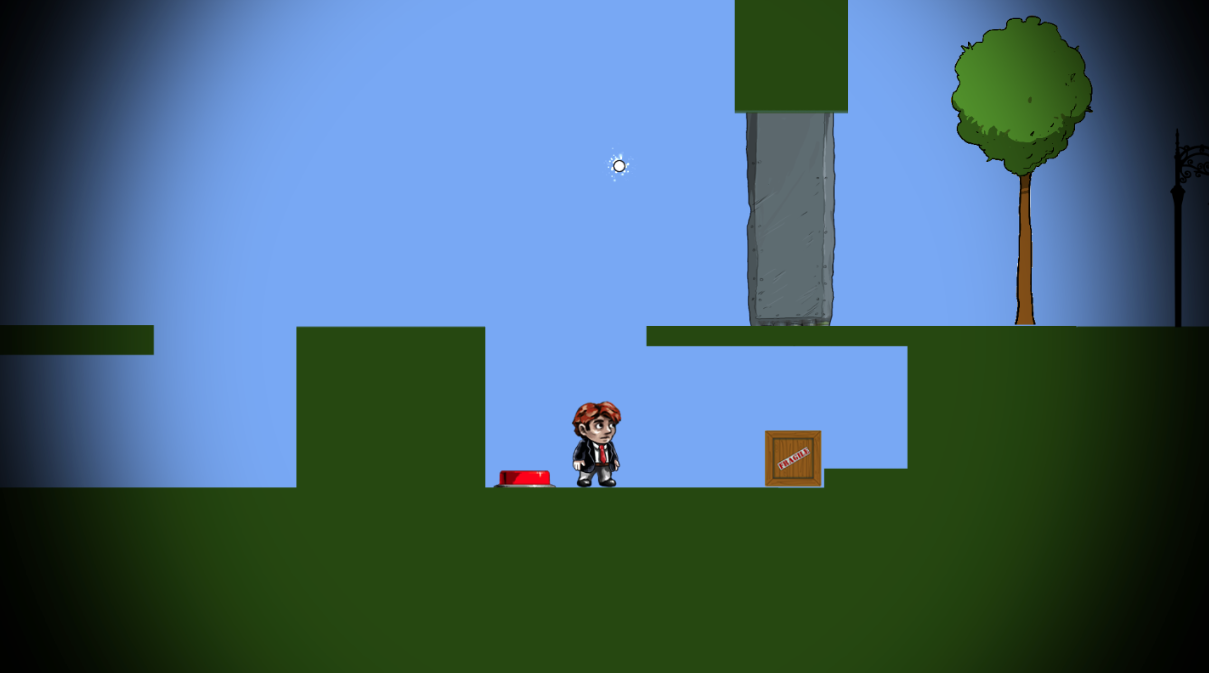
\includegraphics[scale=0.35]{images/development/portaebottone.png}}
\caption{Focus su porta e bottone, dal gameplay di The Magic Lantern.}
\label{fig:portaebottone}
\end{figure}

\subsection{Camera}

\subsection{Altro...}

\section{Strumenti per il testing}

\subsection{Analisi di gameplay}

\subsection{Analisi della fruizione di contenuti Serious}

Per capire quanto i contenuti Serious vengano letti o visti dagli utenti, in vista del testing, sono stati usati gli script \manclass{InformativeManager} e \manclass{TestInformativeManager}. Il salvataggio dei dati avviene tramite un xml dove nel quale si serializza la classe \manclass{InfoSectionContainer}, la quale contiene informazioni riguardo i contenuti (\manclass{InformativeContent} e \manclass{SubContent}) e le relative sezioni (\manclass{InformativeSection}).

I dati salvati riguardano:

\begin{itemize}

\item I tempi, oltre che il numero di volte, impiegati per visualizzare una scheda informativa (cioè un contenuto), avendo pure il dettaglio per sotto-contenuto. Si è tenuto traccia pure del fatto che la scheda sia stata aperta o meno una volta sbloccata o se fosse stata vista in un secondo momento.
\item Poiché sono presenti dei quiz durante i livelli (riguardo i contenuti Serious), si è tenuto traccia del numero di tentativi sbagliati e se alla fine si è risposto in modo corretto.

\end{itemize}

\newpage
